\chapter{Технологический раздел}

\section{Выбор средств программной реализации}
Для реализации комбинированного, а также пошагового и событийного алгоритмов был выбран язык программирования Kotlin и графическая библиотека Swing.

Язык Kotlin был выбран по ряду следующих причин:

\begin{enumerate}
	\item \textbf{Простота и выразительность.} Kotlin предлагает чистый и лаконичный синтаксис, предоставляет множество удобных функций и других инструментов, что значительно упрощает реализацию сложных алгоритмов продвижения модельного времени.
	
	\item \textbf{Высокая производительность.} Kotlin компилируется в байт-код JVM, что позволяет достичь высокой производительности. Это важно для алгоритмов модельного времени, которые требуют обработки больших объемов данных и выполнения вычислительно интенсивных операций.
	
	\item \textbf{Кросс-платформенность.} Код, написанный на Kotlin может работать на различных платформах, включая JVM, Android, JavaScript и Native, что открывает множество возможностей для интеграции реализованных алгоритмов в различные системы.
	
	\item \textbf{Поддержка объектно-ориентированного программирования.} Kotlin предлагает гибкую парадигму программирования, которая позволяет использовать как функциональный, так и объектно-ориентированный стиль программирования. С сущностями поставленной задачи продвижения модельного времени удобнее всего работать как с системой классов.
	
	\item \textbf{Богатая экосистема.} Kotlin имеет широкую и активную экосистему инструментов и библиотек, которые могут быть полезны при реализации алгоритмов. К таким библиотекам относится библиотека Swing, предоставляющая инструменты для создания графического интерфейса.
	
	\item \textbf{Безопасность типов.} Kotlin обеспечивает безопасность типов и проверку на этапе компиляции, что сокращает время отладки и повышает стабильность программного обеспечения.
\end{enumerate}


В свою очередь, библиотека Swing была выбрана в связи со следующими преимуществами:

\begin{enumerate}
	\item \textbf{Кросс-платформенность.} Как и Kotlin, Swing является кросс-платформенной библиотекой, что означает, что приложения, созданные с использованием Swing, могут работать на различных операционных системах. Это обеспечивает широкий охват пользователей и удобство разработки.
	
	\item \textbf{Богатый набор компонентов.} Swing предоставляет обширный набор графических компонентов, что позволяет создавать самые разнообразные интерфейсы в зависимости от требований проекта.

	\item \textbf{Простота использования.} Swing предоставляет интуитивно понятный и простой в использовании API. Kotlin, в свою очередь, предлагает лаконичный и выразительный синтаксис. Сочетание этих двух инструментов делает разработку GUI более удобной и эффективной.
	
	\item \textbf{Хорошая документация и сообщество.} Swing имеет обширную документацию и активное сообщество разработчиков. Это облегчает процесс изучения и получения поддержки, а также предоставляет доступ к множеству ресурсов и примеров кода.
\end{enumerate}


\section{Разработка программного обеспечения}

Полный код разработанного программного обеспечения представлен в приложении.

В рамках данного раздела будут рассмотрены основные классы, необходимые для решения поставленной задачи.

\clearpage
На рисунке \ref{img:uml} представлена диаграмма компонентов разработанного программного обеспечения.

\begin{figure}[h!btp]
	\centering
	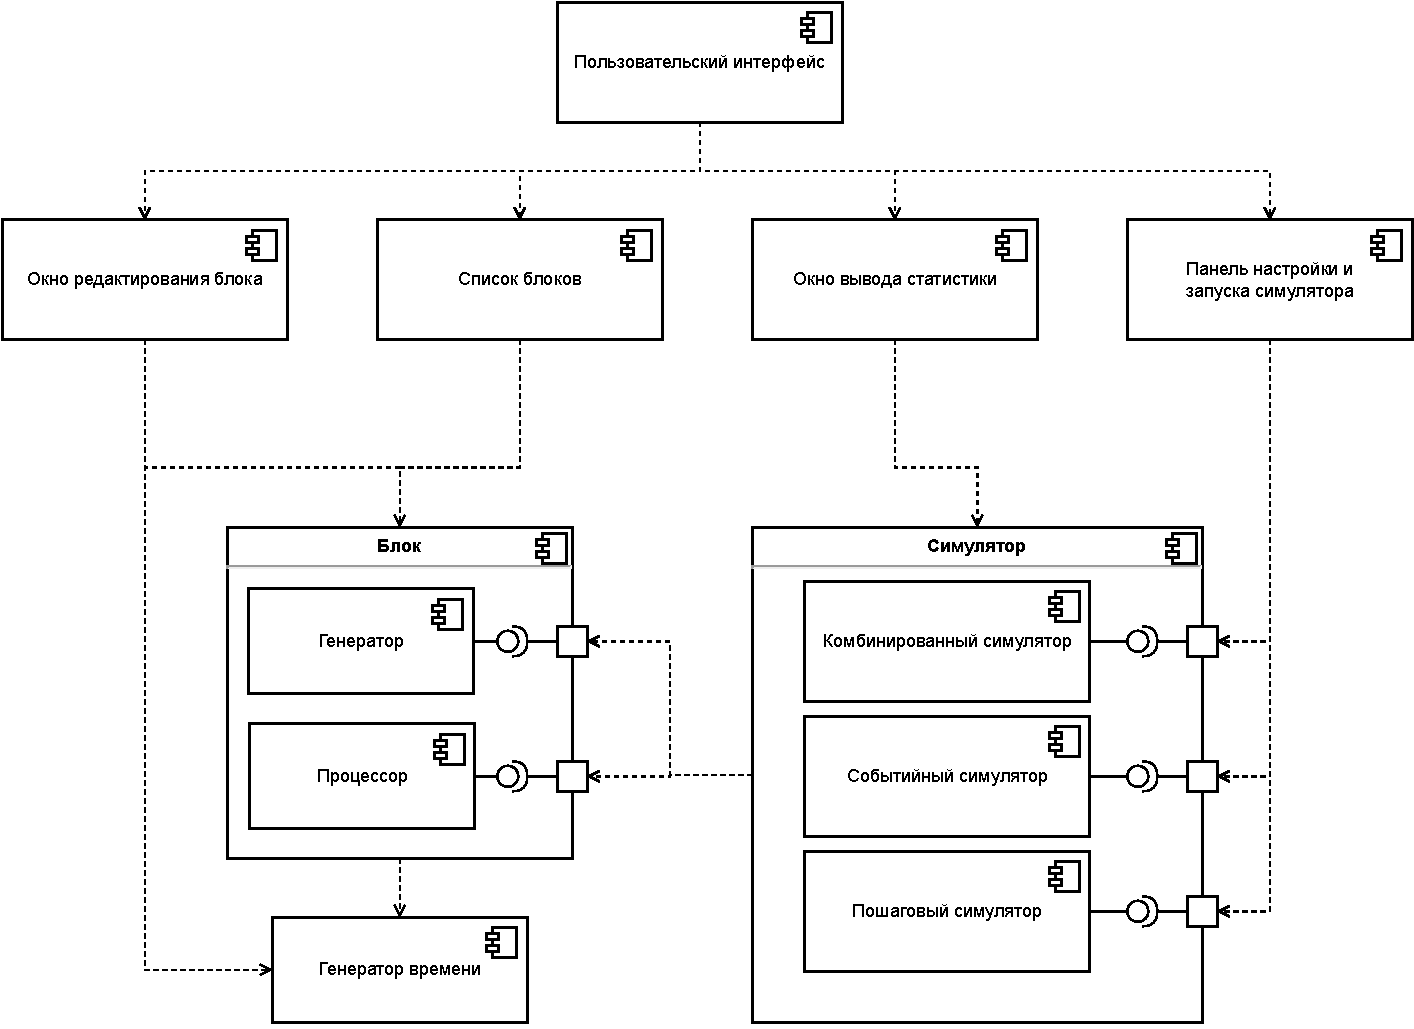
\includegraphics[width=0.7\columnwidth]{inc/img/uml.pdf}
	\caption{Диаграмма компонентов разработанного ПО}
	\label{img:uml}	
\end{figure}


В листинге \ref{lst:DurationGenerator} представлен интерфейс \textbf{DurationGenerator}, который реализуют все классы-генераторы продолжительности, например, класс \textbf{UniformDurationGenerator}, представленный в листинге \ref{lst:UniformDurationGenerator}. Метод $generate$ класса \textbf{UniformDurationGenerator} используется для генерации продолжительность согласно равномерному распределению на основе значений $min$ и $max$, переданных в конструктор. Интерфейс \textbf{DurationGenerator} используется всеми сущностями, реализующими блоки системы, --- процессорами и генераторами, для генерации времени выполнения той или иной операции.
\listingfileKotlin{time/DurationGenerator.kt}{DurationGenerator}{1-100}
\clearpage
\listingfileKotlin{time/UniformDurationGenerator.kt}{UniformDurationGenerator}{1-100}

В листинге \ref{lst:Block} представлен интерфейс \textbf{Block}, который реализуют классы \textbf{Processor} и \textbf{Generator}. Метод $cleanupState$ используется для очистки всей статистики и текущего состояния блока. Метод $currentFinishTime$ --- метод-геттер, используемый для получения времени окончания текущего запущенного процесса. Метод $start$ используется для запуска процесса блока: для генератора --- процесса генерации заявки, для процессора --- процесса обработки заявки.
\clearpage
\listingfileKotlin{simulator/Block.kt}{Block}{1-100}


В листинге \ref{lst:Event} представлен класс \textbf{Event}, описывающий события в моделируемой системе, где $time$ --- время наступления события, $block$ --- блок системы, сгенерировавший событие.
\listingfileKotlin{simulator/Event.kt}{Event}{1-100}


В листинге \ref{lst:Request} представлен класс \textbf{Request}, описывающий заявки в моделируемой системе, где $timeIn$ --- время поступления заявки в с систему, $timeOut$ --- время выхода заявки из системы.
\listingfileKotlin{simulator/Request.kt}{Request}{1-100}


В листингах \ref{lst:Processor-1}, \ref{lst:Processor-2} и \ref{lst:Processor-3} представлен класс \textbf{Processor}, описывающий блок процессора в моделируемой системе. Как уже было сказано выше, он реализует интерфейс \textbf{Block}. Рассмотрим подробнее поля класса:
\begin{itemize}
	\item $durationGenerator$ --- генератор продолжительности обработки заявки;
	\item $receivers$ --- список процессоров-получателей обработанной заявки;
	\item $queue$ --- очередь заявок процессора;
	\item $currentRequest$ --- текущая обрабатываемая заявка;
	\item $currentStartTime$ --- время начала обработки текущей заявки;
	\item $currentFinishTime$ --- время окончания обработки текущей заявки;
	\item $totalRequests$ --- общее количество обработанных заявок;
	\item $totalProcessingTime$ --- общее время работы процессора;
	\item $totalWaitingTime$ --- общее время ожидание заявок в очереди.
\end{itemize}
Помимо этого, класс \textbf{Processor} содержит вложенный класс \textbf{Statistics}, описывающий собираемую по процессору статистику --- общее количество обработанных заявок, среднее время обработки заявки и среднее время ожидания заявки в очереди. Статистика вычисляется с помощью метода $statistics$ на основе полученных за время моделирования значений $totalRequests$, $totalProcessingTime$, $totalWaitingTime$.
\listingfileKotlin{simulator/Processor.kt}{Processor-1}{1-15}
\listingfileKotlin{simulator/Processor.kt}{Processor-2}{16-53}
\listingfileKotlin{simulator/Processor.kt}{Processor-3}{54-91}

В листингах \ref{lst:Generator-1}, \ref{lst:Generator-2} представлен класс \textbf{Generator}, описывающий блок генератора в моделируемой системе. Как уже было сказано выше, он реализует интерфейс \textbf{Block}. Рассмотрим подробнее поля класса:
\begin{itemize}
	\item $durationGenerator$ --- генератор продолжительности генерации заявки;
	\item $receivers$ --- список процессоров-получателей сгенерированной заявки;
	\item $currentRequest$ --- текущая генерируемая заявка;
	\item $currentStartTime$ --- время начала генерации текущей заявки;
	\item $currentFinishTime$ --- время окончания генерации текущей заявки;
	\item $totalRequests$ --- общее количество сгенерированных заявок;
	\item $totalGenerationTime$ --- общее время работы генератора.
\end{itemize}
Помимо этого, класс \textbf{Generator} содержит вложенный класс \textbf{Statistics}, описывающий собираемую по генератору статистику --- общее количество обработанных заявок и среднее время генерации заявки. Статистика вычисляется с помощью метода $statistics$ на основе полученных за время моделирования значений $totalRequests$, $totalGenerationTime$.
\listingfileKotlin{simulator/Generator.kt}{Generator-1}{1-30}
\clearpage
\listingfileKotlin{simulator/Generator.kt}{Generator-2}{31-68}


В листинге \ref{lst:Simulator} представлен интерфейс \textbf{Simulator}, который реализуют классы-симуляторы для пошагового, событийного и комбинированного алгоритмов. В интерфейсе представлен вложенный класс \textbf{Statistics}, описывающий собираемую в процессе моделирования статистику. Класс содержит статистику, собранную со всех процессоров и генераторов, а также общее время выполнения симуляции.
\listingfileKotlin{simulator/Simulator.kt}{Simulator}{1-100}

Листинги классов-симуляторов \textbf{HybridSimulator}, \textbf{TimeBasedSimulator} и \textbf{EventBasedSimulator} приведены в приложении \ref{app:A} и реализуют описанные алгоритмы продвижения модельного времени.

\section{Выводы}
В рамках данного раздела был обоснован выбор программных средств реализации алгоритма. Было разработано программное обеспечение, реализующее комбинированный алгоритм продвижения модельного времени, и описаны ключевые особенности его реализации. Также был разработан пользовательский интерфейс и продемонстрирован пример работы программного обеспечения.